\section{从二分类到多分类}
\label{sec:classification-multiclass}

前面各节的多数推导先以二分类为例。当候选类别超过两个时，还需要规定多个类别怎样竞争：是把多分类问题拆成若干“二选一”的小问题再汇总，还是让所有类别在同一个优化目标里直接竞争。本节把这些公共组合方式集中讲一次，不再散落在各个二分类模型处。硬间隔、软间隔和核方法都能作为构件，但“拆成多个二分类器”与“直接优化多类间隔”会得到不同的训练目标。

现在将标签改为$y_i\in\{1,\ldots,C\}$，其中$C\ge3$，类别索引记为$c$。

\subsection{组合二分类学习器}
\label{sec:classification-combinations}

最直接的推广仍然保留二分类求解器，只改变训练任务的组织方式。

\subsubsection{一对其余（OvR）}
\term{一对其余}（one-vs-rest，OvR）为每个类别$c$构造二分类标签：原标签为$c$时取$+1$，其余取$-1$。训练$C$个实值得分函数$g_c$后，使用
\[
  \hat y(\bm{x})=\argmax_{c\in\{1,\ldots,C\}}g_c(\bm{x}),
\]
并固定平局规则。即使所有得分都为负，或多个类别得分为正，这个最大值规则仍能给出类别。它比较的是独立模型的得分，得分尺度与训练中的类别不平衡可能影响比较，因此通常需要统一预处理、损失约定并评估各类别的错误，若要比较类别后验，还需建立并检验相应的概率映射。

\subsubsection{一对一（OvO）}
\term{一对一}（one-vs-one，OvO）为每对类别$c<c'$训练一个分类器$h_{c,c'}$，仅使用标签为$c$或$c'$的样本，共有$C(C-1)/2$个模型。每个模型在这两个类别之间投一票，预测为
\[
  \hat y(\bm{x})
  =\argmax_{c\in\{1,\ldots,C\}}
     \sum_{c_1<c_2}\mathbb{1}\{h_{c_1,c_2}(\bm{x})=c\}.
\]
其中$c_1,c_2\in\{1,\ldots,C\}$，票数并列时采用预先约定的固定规则，例如选择较小类别编号。不同类别对可能作出不相容的局部判断，投票负责把这些判断汇总成一个输出，并不要求它们对应同一个全局概率模型。

图\ref{fig:classification-svm-multiclass}把四个类别展开成具体训练任务。沿着一列看，一对一中的每个类别只参与三个任务；一对其余中，每个样本都参与四个任务，但只有一个任务把它标为正类。沿着一行看，前者忽略不属于当前类别对的样本，后者把所有其他类别合并为负类。这种训练标签的差异，决定了两个组合器面对的子问题并不相同。

\begin{figure}[htbp]
  \centering
  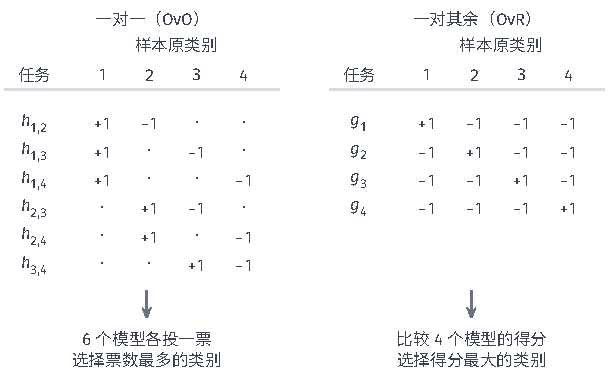
\includegraphics[width=104.027mm]{figures/04-classic-models/00-shared/tikz/classification-svm-multiclass/figure.pdf}
  \caption{四分类任务中的两种二分类组合方式。各行对应一个待训练模型，各列对应样本的原类别；$+1$和$-1$是为该任务重新编码的标签，点号表示该类样本不参与训练。一对一训练6个模型并汇总类别选票，一对其余训练4个模型并比较实值得分。图中给出训练与预测规则，不预设两种方法会产生相同的分类结果。}
  \label{fig:classification-svm-multiclass}
\end{figure}

OvO的模型多、单个训练子问题小，OvR的模型少、每个子问题使用全部样本；总成本因而取决于数据分布和求解器，不能只比较模型个数。

\subsubsection{纠错输出码（ECOC）}

\paragraph{码本与新输入解码}
如果希望组合器能够容忍若干二分类判断错误，可以为每个类别安排一个彼此分离的编码。\term{纠错输出码}（error-correcting output codes，ECOC）将类别$c$表示成长度为$q$的码字$\bm{M}_{c,:}$，其中码本$\bm{M}\in\{-1,+1\}^{C\times q}$的各行互不相同，每列同时含两种符号。码本是在训练之前预先指定的设计结构，不从数据估计。给定训练得到的$q$个二分类器$h_j$，对新输入形成输出码$\bm{h}(\bm{x})=(h_1(\bm{x}),\ldots,h_q(\bm{x}))$，再选择最近的类别码字：
\begin{equation}
  \begin{aligned}
    \hat y(\bm{x})
      &=\argmin_c d_{\mathrm{H}}
          \bigl(\bm{h}(\bm{x}),\bm{M}_{c,:}\bigr),\\
    d_{\mathrm{H}}(\bm{u},\bm{v})
      &=\sum_{j=1}^q\mathbb{1}\{u_j\ne v_j\}.
  \end{aligned}
  \label{eq:classification-svm-ecoc}
\end{equation}
这里的\term{汉明距离}（Hamming distance）就是两个码字不一致的位置数。要表示$C$个不同类别，至少需要$q\ge\lceil\log_2 C\rceil$；加入冗余位的目的，是增大不同类别之间的距离，而不只是增加分类器个数。

\paragraph{编码位训练}
码本设计好后，真正待学的是$q$个二分类器。第$j$列定义一个二分类任务，样本$i$的训练标签为$\bm{M}_{y_i,j}$；在这些人造标签上分别训练得到$h_j$。Dietterich与Bakiri系统研究了这种将多分类转换为多个编码位学习问题的方法\scite{dietterich1995ecoc}。

\paragraph{最近码字解码的纠错条件}
纠错能力可以直接证明。记码本最小类间距离为$\Delta_{\min}$，若真实类别为$c$，输出码与$\bm{M}_{c,:}$相差$e$位，则对任意$c'\ne c$，三角不等式给出
\[
  d_{\mathrm{H}}(\bm{h},\bm{M}_{c',:})
  \ge d_{\mathrm{H}}(\bm{M}_{c,:},\bm{M}_{c',:})-e
  \ge\Delta_{\min}-e.
\]
只要$2e<\Delta_{\min}$，真实码字就比任何其他码字更近。因此至多$\lfloor(\Delta_{\min}-1)/2\rfloor$位错误可以被最近码字解码纠正。这个结论以实际错误位数为条件；若多个二分类器因为相同特征缺陷而同时犯错，冗余编码本身并不能保证错误位数足够小。

\subsubsection{组合方案的尺度与成本}

\paragraph{成员规模与训练成本}
组合尺度上还要计入成本：OvR的$C$个模型、OvO的$C(C-1)/2$个模型、ECOC的$q$个模型，其训练与预测成本随类别数增长。

\paragraph{得分语义与类别概率}
类别不平衡时，OvR每个子问题的正负例比例差异很大，OvO每个子问题只用两类样本，ECOC的编码位还可能把多个类别并为一侧；独立成员的得分尺度与类别概率语义不能直接比较。

\paragraph{整体错误与组合边界}
组合器的风险不能直接取某个成员二分类器的风险，训练中的成员保证若要用于整体分类，还需把错误的二分类比较与最终解码联系起来。

\subsection{联合多类学习}
\label{sec:classification-joint-multiclass}

另一条路线不再训练彼此独立的二分类器，而是直接优化类别之间的竞争关系，在同一目标里学习所有类别的参数。

\subsubsection{多类感知机}
\label{sec:classification-perceptron-multiclass}

\paragraph{类别得分与预测}
对$C$类问题，每类维护一组增广参数$\tilde{\bm{w}}_c=(\bm{w}_c^{\top},b_c)^{\top}$，得分和预测为
\[
  s_c(\bm{x})=\langle\tilde{\bm{w}}_c,\tilde{\bm{x}}\rangle,
  \qquad
  \hat y=\argmax_{c\in\{1,\ldots,C\}}s_c(\bm{x}).
\]
平局仍按最小类别索引处理。这个构造把正确类别的得分与每个竞争类别作比较，也可用\term{Kesler构造}（Kesler construction）把这些比较写成一个扩展空间中的线性可分问题。第$c$类获胜要求$s_c(\bm x)\geq s_j(\bm x)$对每个竞争类成立，平局处再按既定顺序处理。因此每类区域是若干半空间的交，仍是凸区域。它可以表示多类线性分区，却不能在原坐标中把某一类分成被其他类别隔开的多个区域；这种任务需要新的特征或不同的输出表示。

\paragraph{错误触发的参数更新}
遇到$\hat y_i\ne y_i$时，只提高正确类别的参数并降低错误获胜类别的参数：
\begin{equation}
  \label{eq:classification-perceptron-multiclass-update}
  \begin{aligned}
    \tilde{\bm{w}}_{y_i}
      &\leftarrow\tilde{\bm{w}}_{y_i}+\eta\tilde{\bm{x}}_i,\\
    \tilde{\bm{w}}_{\hat y_i}
      &\leftarrow\tilde{\bm{w}}_{\hat y_i}-\eta\tilde{\bm{x}}_i .
  \end{aligned}
\end{equation}
其余类别不变，两个类别的偏置也随各自最后一个分量同时更新。若平局后预测错误，同样更新；若已选择正确类别，则该规则不更新。与二分类中所有零得分均更新的约定不同，这里直接按最终预测是否正确判断。

\paragraph{多类间隔与适用边界}
多类的有限更新保证要求同一个参考参数同时把每个样本的正确类得分，与所有竞争类的得分拉开共同的正间隔；只检查任意一对类别并不足够。样本不可分或没有验证这项条件时，仍应设置停止预算，并选择当前、平均或其他明确的返回规则。

\subsubsection{Crammer–Singer多类SVM}

\paragraph{联合得分与间隔目标}
\term{Crammer--Singer多类SVM}（Crammer--Singer multiclass SVM）要求真实类别得分至少比每个错误类别高一个单位间隔，从而在同一目标中学习所有类别权重。

令$\bm{W}=[\bm{w}_1,\ldots,\bm{w}_C]\in\mathbb{R}^{d\times C}$，使用带偏置的版本$g_c(\bm{x})=\bm{w}_c^{\top}\bm{x}+b_c$，相应优化问题为\scite{crammer2001multiclass}。
\begin{equation}
  \begin{aligned}
    \min_{\bm{W},\bm{b},\bm{\xi}}\quad&
      \frac12\sum_{c=1}^C\lVert\bm{w}_c\rVert_2^2
       +\lambda_{\mathrm{s}}\sum_{i=1}^n\xi_i\\
    \text{s.t.}\quad&
      g_{y_i}(\bm{x}_i)-g_c(\bm{x}_i)\ge1-\xi_i,
      \quad c\ne y_i,\\
    &\xi_i\ge0,\qquad i=1,\ldots,n.
  \end{aligned}
  \label{eq:classification-svm-crammer-singer}
\end{equation}
不使用偏置时固定$\bm{b}=\bm{0}$；使用偏置时，可加$\sum_c b_c=0$去掉共同平移的不识别性。消去松弛变量后，每个样本的损失为$\max\{0,\max_{c\ne y_i}[1+g_c(\bm{x}_i)-g_{y_i}(\bm{x}_i)]\}$，即惩罚最强错误竞争者超过允许差距的程度。预测仍取$\argmax_c g_c(\bm{x})$，并可将权重推广到核特征空间。

\paragraph{模型专属的参数更新与预测}
这一凸目标可以用分解法求对偶，线性形式也可用次梯度训练：对每个样本先找得分最高的错误类别；若它违反单位间隔，损失对正确类权重贡献$-\lambda_{\mathrm s}\bm x_i$，对该竞争类贡献$+\lambda_{\mathrm s}\bm x_i$，其余类为零。累计全部样本的贡献，再加上范数项的梯度$\bm w_c$，沿负方向更新各类权重；偏置只累计损失项的相应标量贡献。最强竞争者并列时任选一个仍给出次梯度。这样，训练直接提高正确类相对于错误竞争者的得分，而不独立拟合每个“该类对其余类”的任务。

\subsubsection{联合目标与原生多类模型的关系}
这一联合目标明确比较了类别之间的相对间隔，OvR则分别比较“该类”与“其余类”。二者的约束数、求解器和数据分解方式不同，训练成本与预测质量也要在相同数据和调参预算下评估。联合建模提供了不同的归纳偏好，并不构成相对于OvO或OvR的普遍性能排序。

Softmax回归（第\ref{sec:classification-softmax}节）本身就是原生多类模型：各类得分经共同分母归一化为概率，直接在一个参数化模型里竞争。组合二分类器与联合多类SVM都不输出归一化概率；若任务需要概率，仍需另行校准（第\ref{sec:classification-calibration}节）。线性OvR与联合多类SVM都按仿射得分的最大值判类，因此每类区域仍是半空间的交。OvO和ECOC先进行若干二分类再解码，各类区域可以由多个分区拼合。这种拼合能够表达单个半空间之外的区域，其能力由可用的二分类划分与解码方式共同决定。

\subsection{大类别集的结构与学习}
\label{sec:classification-large-category-set}

类别特别多时，平坦Softmax要在分母中累加全部类别的指数得分，训练与预测成本随类别数线性增长。下面三种方法分别改变概率的参数化、估计问题或每步比较的负例数量。

\subsubsection{改变概率结构：层次Softmax}

\paragraph{树路径的概率结构}
\term{层次Softmax}（hierarchical softmax）改用树上路径概率的乘积表示一个类别的概率，把一次类别选择拆成沿路径进行的条件选择。这改变了概率的参数化方式，计算某个类别概率时可以沿相应路径展开；类别怎样组织成树，也就成为模型设计的一部分。若需要全部类别概率，计算负担仍然存在，沿路径计算一个类别的概率也不等于已经找到了最高概率类别\scite{goodfellow2016}。

用四个类别构造一个二叉树例子，可以分别看清归一化和搜索。把类别1、2放在根的左子树，类别3、4放在右子树。固定当前输入，设根节点向左的条件概率为$0.6$、向右为$0.4$；到达左子树以后，两片叶的条件概率为$0.5,0.5$；到达右子树以后，两片叶的条件概率为$0.99,0.01$。于是
\[
  \begin{aligned}
    p_1&=0.6\times0.5=0.3,&
    p_2&=0.6\times0.5=0.3,\\
    p_3&=0.4\times0.99=0.396,&
    p_4&=0.4\times0.01=0.004.
  \end{aligned}
\]
四类概率相加为一，因为每个内部节点都把到达它的概率质量完整分给两个孩子。内部节点可以各用一个Logistic模型给出两条分支的条件概率；一旦指定叶子，只需计算沿途节点，不必访问无关分支。在平衡二叉树中，路径长度约为$\log_2C$，不平衡树的路径则可能更长。

\paragraph{沿真实类别路径学习节点参数}
给定类别树后，一条训练记录的真实类别就确定沿途的二元分支标签；训练时把这些节点的Logistic对数概率相加，沿路径求梯度并更新节点参数，无须访问无关分支。设节点$v$的分支概率为$\hat p_v=\sigma(\bm w_v^{\top}\bm x)$，真实路径在该节点指示的分支标签为$y_v\in\{0,1\}$，则该节点对数损失对其参数的梯度为$\partial J/\partial\bm w_v=(\hat p_v-y_v)\bm x$，与二分类Logistic回归逐项同形；只有真实类别路径上的节点收到非零梯度。树的安排固定了哪些类别共享前面的判断，需要作为模型结构选择。

\paragraph{查询对象与计算成本}
这个例子还表明，根处贪心选择较大的左支会错过概率最大的第3类。因此，计算指定类别的概率、找最高概率类别与输出全部类别概率，是三种不同的计算任务。

\subsubsection{估计未归一模型：NCE}

\paragraph{原类别模型与来源辨别结构}
\term{噪声对比估计}（noise-contrastive estimation, NCE）通过区分数据与人为噪声来估计模型，训练时回答一条记录来自数据还是人为噪声，模型参数也决定这项区分的得分。归一化常数可以与模型参数一起估计，避免每一步都对全部候选得分显式求和。它与层次Softmax改变的位置不同：前者改变估计问题，后者把类别概率分解到树上，不能把两者都当作原平坦Softmax公式的计算改写\scite{goodfellow2016}。

沿用新闻主题分类，固定输入$\bm x$，原任务的随机变量$Y$仍表示新闻主题，真实后验为$\eta_c(\bm x)$。现在对每一条真实记录$(\bm x,c^+)$，从已知、可抽样且可求值的噪声分布$q(c\mid\bm x)$独立抽取$k\geq1$个类别，组成噪声配对；这里取$q(c\mid\bm x)>0$覆盖全部候选类别。另引入二元来源标签$D$：真实配对的$D=1$，人为噪声配对的$D=0$。$D$回答配对怎样产生，$Y$回答新闻属于哪个主题，两者不是同一个类别变量。噪声抽样也可能恰好得到$c^+$，这不改变它的来源标签；若排除这种抽样结果，就必须相应改变噪声分布。

\paragraph{来源目标与参数更新}
一条真实记录配$k$条噪声，意味着在混合记录中，两个来源的比例为$1:k$，而不是各占一半。固定同一个$\bm x$后，由贝叶斯公式，真实的来源后验为
\[
  \mathbb P(D=1\mid\bm x,c)
  =\frac{\eta_c(\bm x)}
    {\eta_c(\bm x)+kq(c\mid\bm x)}.
\]
这个式子把原主题后验接到了新增的来源区分任务上。NCE用原模型的非负质量替换未知的$\eta_c$。具体地，保留类别得分$z_{\theta,c}(\bm x)$，另外用可计算函数$\kappa_{\psi}(\bm x)$估计其对数归一化量，定义
\begin{equation}
  \label{eq:classification-nce-source-model}
  \begin{aligned}
    a_{\theta,\psi}(c\mid\bm x)
      &=\exp\{z_{\theta,c}(\bm x)-\kappa_{\psi}(\bm x)\},\\
    h_{\theta,\psi}(\bm x,c)
      &=\frac{a_{\theta,\psi}(c\mid\bm x)}
        {a_{\theta,\psi}(c\mid\bm x)+kq(c\mid\bm x)}\\
      &=\sigma\bigl(z_{\theta,c}(\bm x)-\kappa_{\psi}(\bm x)
                  -\log[kq(c\mid\bm x)]\bigr).
  \end{aligned}
\end{equation}
$\theta$控制原类别得分，$\psi$控制归一化量的函数表示；二者通过$h$共同影响来源预测。训练中$\kappa_{\psi}(\bm x)$不必已经等于$\log\sum_r e^{z_{\theta,r}(\bm x)}$，所以$a_{\theta,\psi}$暂时未必在类别上相加为一；但$h$始终是严格介于零和一之间的二元预测。条件模型的归一化量一般随$\bm x$变化，不能未经假设就用一个共享常数代替。所选$\kappa_{\psi}$的表示与求值也有成本，需要另行规定；若它不能表示所需的归一化函数，估计便会受到这项限制。

令第$i$条真实记录为$(\bm x_i,y_i)$，对应噪声类别为$c^-_{i,1},\ldots,c^-_{i,k}$。既然要提高真实配对来自数据的预测概率，同时提高噪声配对来自噪声的预测概率，每条记录的辅助对数目标就是
\begin{equation}
  \label{eq:classification-nce-objective}
  \begin{aligned}
    J_i^{\mathrm{NCE}}(\theta,\psi)
      &=\log h_{\theta,\psi}(\bm x_i,y_i)\\
      &\quad+\sum_{j=1}^{k}
        \log[1-h_{\theta,\psi}(\bm x_i,c^-_{i,j})].
  \end{aligned}
\end{equation}
对训练记录求和并最大化这个目标，就把原模型参数与归一化参数接入同一项来源分类训练。记$h^+=h_{\theta,\psi}(\bm x_i,y_i)$、$h_j=h_{\theta,\psi}(\bm x_i,c^-_{i,j})$，由$\sigma'(u)=\sigma(u)[1-\sigma(u)]$链式求导，单条记录对参数的梯度骨架为
\[
  \begin{aligned}
    \frac{\partial J_i^{\mathrm{NCE}}}{\partial\theta}
      &=(1-h^+)\frac{\partial z_{\theta,y_i}}{\partial\theta}
        -\sum_{j=1}^{k}h_j\frac{\partial z_{\theta,c^-_{i,j}}}{\partial\theta},\\
    \frac{\partial J_i^{\mathrm{NCE}}}{\partial\psi}
      &=\Bigl[-(1-h^+)+\sum_{j=1}^{k}h_j\Bigr]\,
        \frac{\partial\kappa_{\psi}}{\partial\psi}.
  \end{aligned}
\]
它与二分类Logistic的$(p-y)$梯度同形：真实配对推动$h$靠近1（余量$1-h^+$），噪声配对推动$h$靠近0（余量$h_j$）。每次计算只访问真实类别和抽中的$k$个类别得分，无需在该步显式计算全类别指数和；噪声抽样、噪声概率与$\kappa_{\psi}$的计算成本仍需计入。

\paragraph{估计对象与预测代价}
来源概率与主题概率的数值也不同。例如，三个主题使用均匀噪声，取$k=2$；若某主题的真实后验为$0.6$，则相应来源后验为$0.6/(0.6+2/3)\approx0.474$。因此不能把训练得到的$h$直接当作原主题后验。NCE的统计结论还依赖噪声支持、模型正确指定、归一化函数的可表示性、可识别性以及抽样和优化条件；上述构造没有证明有限样本下$a$已经精确归一化，也没有把辅助目标与原Softmax似然说成同一个目标。若预测接口要求完整的主题概率向量，仍需明确恢复或计算类别归一化，并另外检查校准。

\subsubsection{改用配对目标：负采样}

\paragraph{配对得分与抽样目标}
若每次更新都比较全部其他类别，训练计算会随类别集增大。\term{负采样}（negative sampling）只对抽取的负例建立局部区分目标，减少这一步参与比较的对象。它通常改变原Softmax训练目标，因而应按实际采用的目标解释训练结果；需要类别概率时，也不能直接把局部区分得分当成前面归一化的概率向量\scite{goodfellow2016}。

继续使用一条真实配对与$k$条噪声配对，令$s_\theta(\bm x,c)$为可训练的配对得分。一种常见负采样目标为
\begin{equation}
  \label{eq:classification-negative-sampling-objective}
  \begin{aligned}
    J_i^{\mathrm{NEG}}(\theta)
      &=\log\sigma(s_\theta(\bm x_i,y_i))\\
      &\quad+\sum_{j=1}^{k}
        \log\sigma(-s_\theta(\bm x_i,c^-_{i,j})).
  \end{aligned}
\end{equation}
\paragraph{参数学习与输出范围}
第一项提高真实配对的得分，第二项降低噪声配对的得分。记$s^+=s_\theta(\bm x_i,y_i)$、$s_j=s_\theta(\bm x_i,c^-_{i,j})$。先算单项对得分的导数：由$\partial\log\sigma(s)/\partial s=1-\sigma(s)$，第一项对$s^+$的导数为$1-\sigma(s^+)$；第二项中$\log\sigma(-s_j)$对$s_j$求导，由$\sigma'(u)=\sigma(u)[1-\sigma(u)]$与内层$(-s_j)$的链式得$-(1-\sigma(-s_j))=-\sigma(s_j)$，即$s_j$每增一分，第二项减少$\sigma(s_j)$。因此单条记录对参数的梯度骨架为
\[
  \frac{\partial J_i^{\mathrm{NEG}}}{\partial\theta}
    =(1-\sigma(s^+))\frac{\partial s^+}{\partial\theta}
      -\sum_{j=1}^{k}\sigma(s_j)\frac{\partial s_j}{\partial\theta};
\]
前一项沿提高真实得分的方向更新，后一项$\sigma(s_j)\in(0,1)$沿降低噪声得分的方向更新；若按平均损失写作$L_i=-J_i^{\mathrm{NEG}}$，则负样本项对$s_j$的导数为$+\sigma(s_j)$，与文献中"负例余量"写法一致。
若配对取线性形式$s_\theta(\bm x,c)=\bm w_c^{\top}\bm x$，则$\partial s/\partial\bm w_c=\bm x$，梯度按类别分别累加到$\bm w_{y_i}$与各$\bm w_{c^-_{i,j}}$上。两种方法都用少量配对训练二元区分，但上面的NCE把区分得分明确写成原模型对数质量减去$\log[kq(c\mid\bm x)]$；这个负采样目标的样本项只使用$s_\theta$，没有显式使用该噪声概率修正和归一化函数。噪声分布仍通过抽样影响训练结果，不能理解成负采样与$q$无关。若没有另外建立从$s_\theta$恢复类别概率的关系，$\sigma(s_\theta)$表示的仍是辅助区分预测，不是各主题相加为一的后验；也不能把该目标解释成仅从原Softmax分母删除未抽中的项。
